\documentclass[preprint,11pt]{elsarticle}
\usepackage[margin=2.5cm]{geometry}
\usepackage{sectsty}
\subsectionfont{\normalfont\bfseries}
\usepackage{adjustbox} % For resizing tables
\usepackage{fancyhdr} % Import fancyhdr package
\pagestyle{fancy}
\usepackage[utf8]{inputenc}
\usepackage{amsmath} % For the equation and math symbols
\usepackage{amsfonts} % For math fonts like \mathbb
\usepackage{amssymb} % For additional symbols like \mathbb
\usepackage{pgfplots}
\usepackage{graphicx} % If you want to include images
\usepackage{algorithm}
\usepackage{algpseudocode}

\usepackage{hyperref} % For clickable references
\usepackage{subcaption}
% \usepackage{tabularx} % Allows flexible table widths

\newcommand{\vw}{\mathbf{w}} % or \vec{w} for arrow notation

\title{\rule{\linewidth}{0.5mm} \\ \Large{\textbf{Online Graph Dictionary Learning}}\\
\rule{\linewidth}{0.5mm}}
\author{Cedric Vincent-Cuaz$^1$, Titouan Vayer$^2$, Remi Flamary$^3$, Marco Corneli$^4$, Nicolas Courty$^5$}


\begin{document}

% \begin{center}
    
%     \rule{\linewidth}{0.5mm} \\[0.4cm] 
%     \Large{\textbf{Online Graph Dictionary Learning}} \\[0.4cm]
%     \rule{\linewidth}{0.5mm} \\[1cm]  
%     \textbf{Cedric Vincent-Cuaz}$^1$, \hspace{0.1cm} \textbf{Titouan Vayer}$^2$, \hspace{0.5mm} \textbf{Remi Flamary}$^3$, \hspace{0.5mm} \textbf{Marco Corneli}$^4$, \hspace{0.5mm} \textbf{Nicolas Courty}$^5$ \\[0.5cm]
    
    
% \end{center}


\begin{abstract}
    Dictionary learning is a key tool for representation learning that explains data as a linear combination of a few basic elements. Yet, this analysis is not easily applicable in the context of graph learning, as graphs usually belong to different metric spaces. We fill this gap by proposing a new online Graph Dictionary Learning approach, which uses the Gromov-Wasserstein divergence for the data fitting term. In our work, graphs are encoded through their nodes’ pairwise relations and modeled as a convex combination of graph atoms, {\em i.e.}, dictionary elements, estimated through an online stochastic algorithm that operates on a dataset of unregistered graphs with potentially different numbers of nodes. Our approach naturally extends to labeled graphs and is completed by a novel upper bound that can be used as a fast approximation of Gromov-Wasserstein in the embedding space. We provide numerical evidence showing the interest of our approach for unsupervised embedding of graph datasets and for online graph subspace estimation and tracking.
\end{abstract}

\maketitle
\fancyhf{} % Clear all header and footer fields
\fancyhead[C]{\textbf{Online Graph Dictionary Learning}} % Centered title at the top of every page
\fancyfoot[C]{\thepage} % Centered page number at the bottom



\section{Introduction}
    In recent years, the challenge of building machine learning algorithms that can handle structured data like graphs has gained considerable interest. Applications range from molecule compounds, brain connectivity, and social networks, to time series and image analysis. A key difficulty arises due to the non-vectorial nature of graphs, requiring specialized models. While neural networks have shown success in end-to-end approaches with labeled data, unsupervised learning remains a significant challenge, especially when data is continuously generated through streams. Tackling the non-stationarity of such processes is complex, as seen in dynamic connectivity and network science. In this context, this work proposes an online graph dictionary learning method to handle graphs with varying structures and nodes.

\section{\textbf{Online Graph Dictionary Learning}}
    \subsection{{\textbf{(Fused)Gromov-Wasserstein for graph simirality}}}
    
A graph \( G^X \) with \( N^X \) nodes, can be regarded as a tuple \( (C^X, h^X) \) where \( C^X \in \mathbb{R}^{N^X \times N^X} \) is a matrix that encodes a notion of similarity between nodes and \( h^X \in \Sigma^{N^X} \) is a histogram, or equivalently a vector of weights which models the relative importance of the nodes within the graph. Without any prior knowledge, uniform weights can be chosen so that \( h^X = \frac{1}{N^X} 1_{N^X} \). The matrix \( C^X \) carries the neighborhood information of the nodes and, depending on the context, it may designate the adjacency matrix, the Laplacian matrix \cite{maretic2019got}, or the matrix of the shortest-path distances between the nodes \cite{bavaud2010euclidean}. 

Let us now consider two graphs \( G^X = (C^X, h^X) \) and \( G^Y = (C^Y, h^Y) \), of potentially different orders (\textit{i.e.} \( N^X \neq N^Y \)). The GW2 distance between \( G^X \) and \( G^Y \) is defined as the result of the following optimization problem:

\begin{equation}
    \min_{T \in \mathcal{U}(h^X, h^Y)} \sum_{ijkl} \left( C^X_{ij} - C^Y_{kl} \right)^2 T_{ik} T_{jl}
\end{equation}

where

\[
    \mathcal{U}(h^X, h^Y) := \left\{ T \in \mathbb{R}^{N^X \times N^Y}_+ \mid T1_{N^Y} = h^X, T^T 1_{N^X} = h^Y \right\}
\]

is the set of couplings between \( h^X \) and \( h^Y \). The optimal coupling \( T \) of the GW problem acts as a probabilistic matching of nodes which tends to associate pairs of nodes that have similar pairwise relations in \( C^X \) and \( C^Y \), respectively. In the following, we denote by \( GW_2^2(C^X, C^Y, h^X, h^Y) \) the optimal value of equation (1) or by \( GW_2^2(C^X, C^Y) \) when the weights are uniform.

The previous framework can be extended to graphs with node attributes (typically \( \mathbb{R}^d \) vectors). In this case, we use the Fused Gromov-Wasserstein distance (FGW) \cite{Vayer2018, Vayer2019} instead of GW. More precisely, a labeled graph \( G^X \) with \( N^X \) nodes can be described this time as a tuple \( G^X = (C^X, A^X, h^X) \) where \( A^X \in \mathbb{R}^{N^X \times d} \) is the matrix of all features. Given two labeled graphs \( G^X \) and \( G^Y \), FGW aims at finding an optimal coupling by minimizing an OT cost which is a trade-off of a Wasserstein cost between the features and a GW cost between the similarity matrices. For the sake of clarity, we detail our approach in the GW context and refer the reader to the supplementary material for its extension to FGW.


\subsection{Linear embedding and GW unmixing}

\textbf{Linear modeling of graphs} We propose to model a graph  as a weighted sum of pairwise relation matrices. More precisely, given a graph \( G = (C,h) \) and a dictionary \( \{\overline{C}_s\}_{s \in [S]} \), we want to find a linear representation \( G \approx \sum_{s \in [S]} w_s \overline{C}_s \) of the graph \( G \), as faithful as possible. The dictionary is made of pairwise relation matrices of graphs with order \( N \). Thus, each \( \overline{C}_s \in S_{N}(\mathbb{R}) \) is called an \emph{atom}, and $\vw=(w_{s})_{s \in [S]} \in \Sigma_S$ is referred as
	\emph{embedding} and denotes the coordinate of the graph \( G \) in the dictionary, as illustrated in Fig. 1. We rely on the Gromov-Wasserstein (GW) distance to assess the quality of our linear approximation and propose to minimize it to estimate its optimal embedding. In addition to being interpretable thanks to its linearity, we also propose to promote sparsity in the weights \( w \) similarly to sparse coding \cite{chen2001atomic}. Finally, note that when the pairwise matrices \( \overline{C} \) are adjacency matrices and the dictionary atoms have components in \([0, 1]\), the model \( \sum_{s \in [S]} w_s \overline{C}_s \) provides a matrix whose components can be interpreted as probabilities of connection between the nodes.


\textbf{Gromov-Wasserstein unmixing} We first study the unmixing problem that consists in projecting a graph onto the linear representation discussed above, i.e., to estimate the optimal embedding \( w \) of a graph \( G \). The unmixing problem can be expressed as the minimization of the GW distance between the similarity matrix associated with the graph and its linear representation in the dictionary:
\begin{equation}
    \min_{\vw \in \Sigma_S}\quad GW^2_2\left(\mC, \sum_{s \in [S]} w_s \overline{\mC}_s\right) - \lambda \|\vw\|^2_2 \label{eq:unmix}
\end{equation}   
	
	
where \( R^+ \) induces a negative quadratic regularization promoting sparsity on the simplex as discussed in \cite{li2016methods}.

\textbf{Algorithm 1: BCD for unmixing problem}

\begin{algorithm}[H]
\caption{BCD for unmixing problem 2}
\begin{algorithmic}
\State Initialize $w = \frac{1}{S} \mathbf{1}_S$
\Repeat
\State Compute OT matrix $T$ of GW$^2(C, \Sigma, \overline{w}_s C_s)$, with CG algorithm (Vayer et al., 2018, Alg.1 & 2).
\State Compute the optimal $w$ solving equation 2 for a fixed $T$ with CG algorithm.
\Until{convergence}
\end{algorithmic}
\end{algorithm}

In order to solve the non-convex problem in equation (2), we propose to use a Block Coordinate Descent (BCD) algorithm \cite{tseng2001convergence}. The BCD works by alternatively updating the OT matrix of the GW distance and the embeddings \( w \). When \( w \) is fixed, the problem is a classical GW, which is a non-convex quadratic program. We solve it using a Conditional Gradient (CG) algorithm \cite{jaggi2013revisiting} based on \cite{vayer-optimal-nodate}. Note that the use of the exact GW instead of a regularized proxy allowed us to keep a sparse OT matrix as well as to preserve high-frequency components of the graph, as opposed to regularized versions of GW \cite{peyre2016gromov,solomon_entropic_2016,xu2019gromov} that promote dense OT matrices and lead to smoothed/averaged pairwise matrices. For a fixed OT matrix \( T \), the problem of finding \( w \) is a non-convex quadratic program and can also be tackled with a CG algorithm. Note that for non-convex problems, the CG algorithm is known to converge to a local stationary point \cite{lacoste-julien-convergence-2016}. In practice, we observed a typical convergence of the CG in a few tens of iterations. The BCD itself converges in less than 10 iterations.

\textbf{Fast upper bound for GW} Interestingly, when two graphs belong to the linear subspace defined by our dictionary, there exists a proxy of the GW distance using a dedicated Mahalanobis distance as described in the next proposition:

\textbf{Proposition 1} For two embedded graphs with embeddings \( w^{(1)} \) and \( w^{(2)} \), assuming they share the same weights \( h \), the following inequality holds:

\begin{equation}
    GW^2\left(\sum_{s \in [S]} w^{(1)}_s C_s, \sum_{s \in [S]} w^{(2)}_s C_s\right) \leq \|w^{(1)} - w^{(2)}\|_M
\end{equation}

where \( M_{pq} = D_h C_p C_q D_h \) and \( D_h = \text{diag}(h) \). \( M \) is a positive semi-definite matrix, hence engenders a Mahalanobis distance between embeddings. 

As detailed in the supplementary material, this upper bound is obtained by considering the GW cost between the linear models calculated using the admissible coupling \( D_h \). The latter coupling assumes that both graph representations are aligned and therefore is a priori suboptimal. As such, this bound is not tight in general. However, when the embeddings are close, the optimal coupling matrix should be close to \( D_h \), so that Proposition 1 provides a reasonable proxy to the GW distance in our embedding space. In practice, this upper bound can be used to efficiently compute pairwise kernel matrices or to retrieve the closest samples (see numerical experiments).

\section{Numerical experiments}
    \subsection{GDL on real data for clustering and classification}
    \textbf{Results and interpretation}   Clustering results can be
 seen in Table 1. The mean RI and its standard deviation are
 reported for each dataset and method. Our model outper-
forms or is at least comparable to the state-of-the-art OT
 based approaches for most of the datasets. Results show
 that the negative quadratic regularization proposed with our
 models brings additional gains in performance. Note that for
 this benchmark, we considered a fixed batch size for learning our models on labeled graphs, which turned out to be a
 limitation for the dataset ENZYMES. Indeed, comparable
 conclusions regarding our models performance have been
 observed by setting a higher batch size for this latter dataset and are reported in the supplementary material. This might be due to both a high number of heterogeneous classes and a high structural diversity of labeled graphs inside and among classes. We illustrate in Fig. 5 the interest of the extension of GDL with estimated weights for IMDB-M dataset. We can see in the center-left part of the figure that, without estimating the weights, GDL can experience difficulties producing a model that preserves the global structure of the graph because of the uniform weights on the nodes. In opposition, simultaneously estimating the weights brings a more representative modeling (in the GW sense), as illustrated in the centered right columns. The weights estimation can re-balance and even discard non-relevant nodes, in the vein of attention mechanisms. We report in the supplementary material a companion study for clustering tasks which further supports our extension concerning the learning of node weights.
\begin{table}[ht]
\centering
\caption{Clustering: Rand Index computed for benchmarked approaches on real datasets}
\scriptsize
\begin{tabular}{|c|c|c|c|c|c|c|c|c|c|}
\hline
\multicolumn{1}{|c|}{MODELS} & \multicolumn{2}{c|}{NO ATTRIBUTE} & \multicolumn{2}{c|}{DISCRETE ATTRIBUTES} & \multicolumn{4}{c|}{REAL ATTRIBUTES} \\ \hline
MODELS & IMDB-B & IMDB-M & MUTAG & PTC-MR & BZR & COX2 & ENZYMES & PROTEIN \\
\hline
GDL (ours) & 51.32(0.30) & 55.08(0.28) & 70.02(0.29) & 51.53(0.36) & 62.59(1.68) & 58.39(0.52) & 66.97(0.93) & 60.22(0.30) \\
GDLA (ours) & 51.64(0.59) & 55.41(0.20) & 70.89(0.11) & 51.90(0.54) & 66.42(1.96) & 59.48(0.68) & 66.79(1.12) & 60.49(0.71) \\
\hline
GWF-r & 51.24(0.02) & 55.54(0.03) & 68.83(1.47) & 51.44(0.52) & 52.42(2.48) & 56.84(0.41) & 72.13(0.19) & 59.96(0.09) \\
GWF-f & 50.47(0.34) & 54.01(0.37) & 58.96(1.91) & 50.87(0.79) & 51.65(2.96) & 52.86(0.53) & 71.64(0.31) & 58.89(0.39) \\

GW-k & 50.32(0.02) & 53.65(0.07) & 57.56(1.50) & 50.44(0.35) & 56.72(0.50) & 52.48(0.12) & 66.33(1.42) & 50.08(0.01) \\
SC & 50.11(0.10) & 54.40(9.45) & 50.82(2.71) & 50.45(0.31) & 42.73(7.06) & 41.32(6.07) & 70.74(10.60) & 49.92(1.23) \\
\hline
\end{tabular}
\end{table}

\begin{figure}[ht]
    \centering
    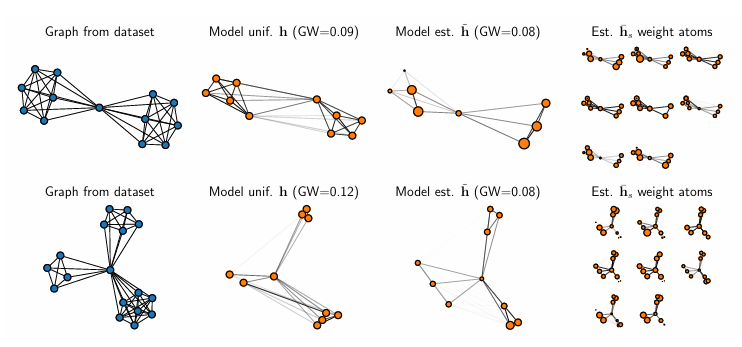
\includegraphics[width=\textwidth]{Images/newmodel.png} % Adjust the path
    \caption{Modeling of two real life graphs from IMDB-M with our GDL approaches with 8 atoms of order 10. (left) original graphs from the dataset, (center left) linear model for GDL with uniform weights as in equation 4, (center right) linear model for GDL with estimated weights as in equation 6 and (right) different hs on the estimated structure.
}
    \label{fig:image_1}
\end{figure}



\begin{figure}[htbp]
    \centering
    \begin{subfigure}[b]{0.45\textwidth}
        \centering
        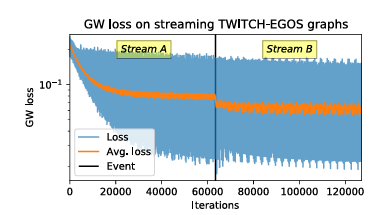
\includegraphics[width=\textwidth]{Images/1.png}
        % \caption{Image 1 Title}
      
        \label{fig:image1}
        
    \end{subfigure}
    \hfill
    \begin{subfigure}[b]{0.45\textwidth}
        \centering
        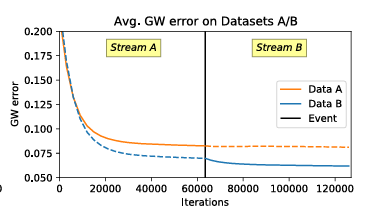
\includegraphics[width=\textwidth]{Images/2.png}
        % \caption{Image 2 Title}
        \label{fig:image2}
      
    \end{subfigure}

    \vspace{1em}

    \begin{subfigure}[b]{0.45\textwidth}
        \centering
        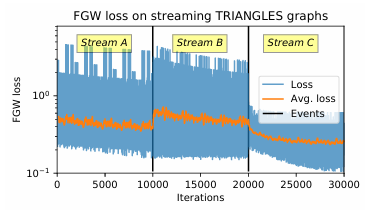
\includegraphics[width=\textwidth]{Images/3.png}
        % \caption{Image 3 Title}
        \label{fig:image3}
       
    \end{subfigure}
    \hfill
    \begin{subfigure}[b]{0.45\textwidth}
        \centering
        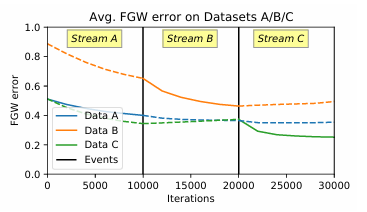
\includegraphics[width=\textwidth]{Images/4.png}
        % \caption{Image 4 Title}
        \label{fig:image4}
        
    \end{subfigure}

    \caption{\textbf{Online GD London dataset TWITCH - EGOS with 2 atoms of 14 nodes each (top) and on TRIANGLES with 4 atoms of 17 nodes each (bottom).
}}
    \label{fig:combined}
\end{figure}
\newpage

\bibliography{citation}
\bibliographystyle{ieeetr}


\end{document}






    
\end{document}

\end{document}
